\subsection{Known Approximations for Transcendental Functions}
Many methods to compute transcendental functions implemented in computer hardware and software libraries rely on direct knowledge of the function arguments. Several such approaches include using the CORDIC (coordinate rotation digital computer), pseudo-division and pseudo-multiplication algorithms \cite{walther_cordic_2000}, as well as using minimax polynomials, which are determined numerically using the Remez algorithm \cite{harrison_computation_1999}. These algorithms, while efficient, rely on table lookups, which cannot be done in a privacy-preserving system where the function arguments cannot be directly determined.

We must therefore rely on other methods, such as using the Taylor series expansions of these functions. While also in common use, not all Taylor series expansions have a convenient radius of convergence. To circumvent this, we can rely on an approach presented by Khattri in \cite{khattri_new_2009} to obtain closed form approximations to functions by approximating related integrals.

Khattri presents the following method to approximate the function $f(x)=\log(1+x)$.
Let $x = 1/n$ and consider the integral
\begin{align}
	\label{eq:log_integral}
	\int_{n}^{n+1}{\frac{1}{x}\diff x}=\log{\left(1+\frac{1}{n}\right)}.
\end{align}

This integral can be approximated using the five-point Gauss-Legendre quadrature rule \cite{kythe_quadrature_2002}. We first convert the integral to an integral over the interval $[-1,1]$ using the following transformation:
\begin{align*}
	\int_a^b{f(x)\diff x}
	&= \frac{b-a}{2}\int_{-1}^{1}{f\left(\frac{b-a}{2}x+\frac{a+b}{2}\right)\diff x}.
\end{align*}
Then, we approximate the integral using the following summation:
\begin{align*}
	\int_{-1}^{1}{f(x)\diff x} &= \sum_{i=1}^{5}{w_if(x_i)},
\end{align*}
where
\begin{multicols}{2}
	\noindent
	\begin{align*}
		w_1 &= 0\\
		w_2 &= \frac{1}{21}\sqrt{245-14\sqrt{70}}\\
		w_3 &= -\frac{1}{21}\sqrt{245-14\sqrt{70}}\\
		w_4 &= \frac{1}{21}\sqrt{245+14\sqrt{70}}\\
		w_5 &= -\frac{1}{21}\sqrt{245+14\sqrt{70}}
	\end{align*}
	\columnbreak
	\begin{align*}
		x_1 &= \frac{128}{225}\\
		x_2 &= \frac{1}{900}\left( 322 + 13\sqrt{70}\right)\\
		x_3 &= \frac{1}{900}\left( 322 + 13\sqrt{70}\right)\\
		x_4 &= \frac{1}{900}\left( 322 - 13\sqrt{70}\right)\\
		x_5 &= \frac{1}{900}\left( 322 - 13\sqrt{70}\right)
	\end{align*}
\end{multicols}
Applying this procedure to the integral in equation \ref{eq:log_integral} yields the following approximation:
\begin{equation}\label{eq:standard_logarithm_quadrature}
	\log(1+x) =
	\frac{137x^5 + 2310x^4 + 9870x^3 + 15120x^2 + 7560x}
	{30x^5 + 900x^4 + 6300x^3 + 16800x^2 + 18900x + 7560}.
\end{equation}
While the closed form approximation presented by Khattri (equation \ref{eq:standard_logarithm_quadrature}) is accurate for values of $x$ near zero, it diverges from $\log{(1+x)}$ significantly for large values of $x$, as shown in figure \ref{fig:standard_logarithm_quadrature}.
\begin{figure}[!ht]
		\centering
		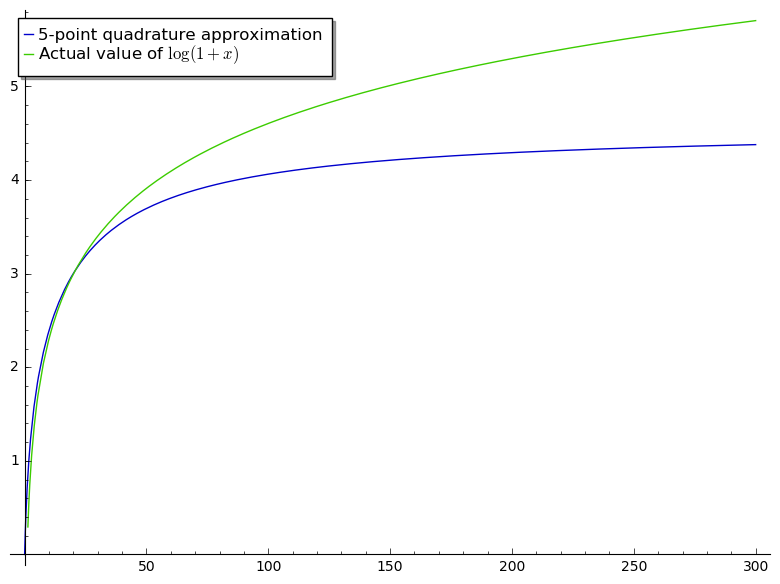
\includegraphics[width=.8\linewidth]{figures/StandardQuadrature.png}
		\caption{Graph of $\log{(1+x)}$ and the approximation in equation \ref{eq:standard_logarithm_quadrature}}
		\label{fig:standard_logarithm_quadrature}
\end{figure}

However, the quadrature approach presented by Khattri allows us to approximate the logarithm in a larger range than is possible with the Taylor series, as the Taylor series of $\log(1+x)$ has an interval of convergence of $[-1,1]$.
